%__________________________________
\chapter{Data Extraction Tools}

Uintah offers a number of tools for accessing data stored in Uintah
Data Archives (``UDAs").  Because the format of Uintah data is
specific to the framework, these tools allow a user to quickly extract
data, which can then either be postprocessed within that tool (simple
modification of the source code may be necessary), postprocessed with
external software such as Matlab or Octave, or simply plotted with,
e.g. gnuplot.  These tools are not compiled automatically when ``make
sus'' is issued.  To compile them cd to ``opt/StandAlone/tools'' and
issue ``make''.  These tools are described below.

\section{puda}

The command line extraction utility \tt puda \normalfont (for ``parse
Uintah data archive") has a number of uses.  For example, it may be
used to extract a subset of particle data from a UDA.  Once the
extraction tools have been compiled, the puda executable will be
located in \tt opt/StandAlone/tools/puda/. \normalfont If the
executable is run with no additional command line arguments, the
following usage information will be displayed:

\begin{lstlisting}
Usage: puda [options] <archive file>

Valid options are:
  -h[elp]
  -timesteps
  -gridstats
  -listvariables
  -varsummary
  -jim1
  -jim2
  -partvar <variable name>
  -asci
  -tecplot <variable name>
  -no_extra_cells     (Excludes extra cells when iterating over cells.
                       Default is to include extra cells.)
  -cell_stresses
  -rtdata <output directory>
  -PTvar
  -ptonly             (prints out only the point location
  -patch              (outputs patch id with data)
  -material           (outputs material number with data)
  -NCvar <double | float | point | vector>
  -CCvar <double | float | point | vector>
  -verbose            (prints status of output)
  -timesteplow <int>  (only outputs timestep from int)
  -timestephigh <int> (only outputs timesteps up to int)
  -matl,mat <int>         (only outputs data for matl)
*NOTE* to use -PTvar or -NVvar -rtdata must be used
*NOTE* ptonly, patch, material, timesteplow, timestephigh are used in conjunction with -PTvar.
\end{lstlisting}

As an example of how to use \tt puda, \normalfont suppose that one
wanted to know the locations of all particles at the last archived
timestep for the \lstinline!const_test_hypo.uda!. First one may
wish to know how many timesteps have been archived.  This could be
accomplished by:

\begin{lstlisting}
 puda -timesteps const_test_hypo.uda
\end{lstlisting}
The resulting terminal output would be:
\begin{lstlisting}
Parsing const_test_hypo.uda/index.xml
There are 11 timesteps:
1: 1.8257001926347728e-05
548: 1.0012914931998474e-02
1094: 2.0005930425875382e-02
1640: 3.0015616802173569e-02
2184: 4.0005272397960444e-02
2728: 5.0011587657447343e-02
3271: 6.0016178181543284e-02
3812: 7.0000536667661845e-02
4353: 8.0001537138146825e-02
4893: 9.0000702723306208e-02
5433: 1.0001655973087024e-01
\end{lstlisting}

These represent all of the timesteps for which data has been archived.
Suppose now that we wish to know what the stress state is for all
particles (in this case two) at the final archived timestep.  For this
one could issue:

\begin{lstlisting}
puda -partvar p.stress -timesteplow 10 -timestephigh 10 const_test_hypo.uda
\end{lstlisting}

The resulting output is:

\begin{lstlisting}
Parsing const_test_hypo.uda/index.xml
1.00016560e-01 1 0 281474976710656 -2.72031498e-10 -1.05064208e-26 -2.53781271e-08 -1.05064208e-26 -2.72031498e-10 -1.23584688e-09 -2.53781271e-08 -1.23584688e-09 1.63840079e-07
1.00016560e-01 1 1 0 1.93256890e-13 6.56787331e-18 1.85514400e-14 6.56787331e-18 2.24310469e-13 1.85519650e-14 1.85514400e-14 1.85519650e-14 -3.20052991e+06
\end{lstlisting}

The first column is the simulation time, the third column is the
material number, the fourth column is the particle ID, and the
remaining nine columns represent the components of the Cauchy stress
tensor ($ \sigma_{11}$,$\sigma_{12}$,$\sigma_{13}$, ...,
$\sigma_{32}$,$\sigma_{33}$).  If desired, the terminal output can be
redirected to a text file for further use.

\section{partextract}

The command-line utility \tt partextract \normalfont may be used to
extract data from an individual particle.  To do this you first need
to know the ID number of the particle you are interested in.  This may
be done by using the puda utility, or the visualization tools.  Once
the extraction tools have been compiled, the partextract utility
executable will be located in \tt /opt/StandAlone/tools/extractors/
\normalfont.  If the executable is run without any arguments the
following usage guide will be displayed in the terminal:

\begin{lstlisting}
No archive file specified
Usage: partextract [options] <archive file>

Valid options are:
  -mat <material id>
  -partvar <variable name>
  -partid <particleid>
  -part_stress [avg or equiv or all]
  -part_strain [avg/true/equiv/all/lagrangian/eulerian]
  -timesteplow [int] (only outputs timestep from int)
  -timestephigh [int] (only outputs timesteps upto int)
\end{lstlisting}

As an example of how to use the partextract utility, suppose we wanted
to find the velocity at every archived timestep for the particle with
ID 281474976710656 (found above using puda) in the
``\lstinline!const_test_hypo.uda!'' file (src/StandAlone/inputs/MPM).  The
appropriate command to issue is:

\begin{lstlisting}
partextract -partvar p.velocity -partid 281474976710656 const_test_hypo.uda
\end{lstlisting}

The output to the terminal is:

\begin{lstlisting}
Parsing const_test_hypo.uda/index.xml
1.82570019e-05 1 0 281474976710656 0.00000000e+00 0.00000000e+00 -1.00000000e-02
1.00129149e-02 1 0 281474976710656 -1.03554318e-19 -1.03554318e-19 -1.00000000e-02
2.00059304e-02 1 0 281474976710656 -1.99388121e-19 -1.99388121e-19 -1.00000000e-02
	.
	.
	.
\end{lstlisting}

It is noted that if the stress tensor is output using the partextract utility, the output format is different than for the puda utility.  The partextract utility only outputs the six independent components instead of all nine.  For example, if we use partextract to get the stress tensor for the same particle as above at the last archived timestep only, the output is:

\begin{lstlisting}
partextract -partvar p.stress -partid 281474976710656 -timesteplow 10 -timestephigh 10 const_test_hypo.uda
Parsing const_test_hypo.uda/index.xml
1.00016560e-01 1 0 281474976710656 -2.72031498e-10 -1.05064208e-26 -2.53781271e-08 -1.05064208e-26 -2.72031498e-10 -1.23584688e-09 -2.53781271e-08 -1.23584688e-09 1.63840079e-07
\end{lstlisting}

Compare this output with the output from puda above.  Notice that the
ordering of the six independent components of the stress tensor for
partextract are $\sigma_{11}$,$\sigma_{22}$, $\sigma_{33}$,
$\sigma_{23}$, $\sigma_{13}$ , $\sigma_{12}$.

\section{lineextract}

Lineextract is used to extract an array of data from a region of a
computational domain. Data can be extracted from a point, along a
line, or from a three dimensional region and then stored as a variable
for ease of post processing.

Usage: \begin{lstlisting}
./lineextract [options] -uda <archive file>

Valid options are:
 -h,        --help
 -v,        --variable:      <variable name>
 -m,        --material:      <material number> [defaults to 0]
 -tlow,     --timesteplow:   [int] (sets start output timestep to int) [defaults to 0]
 -thigh,    --timestephigh:  [int] (sets end output timestep to int) [defaults to last timestep]
 -timestep, --timestep:      [int] (only outputs from timestep int) [defaults to 0]
 -istart,   --indexs:        <x> <y> <z> (cell index) [defaults to 0,0,0]
 -iend,     --indexe:        <x> <y> <z> (cell index) [defaults to 0,0,0]
 -l,        --level:         [int] (level index to query range from) [defaults to 0]
 -o,        --out:           <outputfilename> [defaults to stdout]
 -vv,       --verbose:       (prints status of output)
 -q,        --quiet:         (only print data values)
 -cellCoords:                (prints the cell centered coordinates on that level)
 --cellIndexFile:             <filename> (file that contains a list of cell indices)
                                  [int 100, 43, 0]
                                  [int 101, 43, 0]
                                  [int 102, 44, 0]
\end{lstlisting}

The following example shows the usage of lineextract for extracting
density data at the 60th computational cell in the x-direction,
spanning the width of the domain in the y-direction (0 to 1000), at
timestep, 7, (note ``timestep" actually refers to the seventh data
dump, not necessarily the seventh timestep in the simulation. The
variable containing the density data within the uda is ``\lstinline!rho_CC!," and
the output variable that will store the data for post processing is
``rho."
\begin{lstlisting}
./lineextract -v rho_CC  -timestep 7 -istart 60 0 0 -iend 60 1000 0 -m 1 -o rho -uda test01.uda.000
\end{lstlisting}

%__________________________________
\section{\lstinline!compute_Lnorm_udas!}
\lstinline!Compute_Lnorm_udas! computes the $L_1$, $L_2$ and $L_\infty$
norms for each variable in two udas.  This utility is useful in
monitoring how the solution differs from small changes in either the
solution tolerances, input parameters or algorithmic changes.  You can
also use it to test the domain size influence.  The norms are computed
using:
%
\begin{equation}
  d[i] = |uda_1[i] - uda_2[i]|
\end{equation}
%
\begin{equation}
  L_1 = \frac{\raise1.5pt\hbox{$\sum_i^{\rm{All Cells}}$}d[i]}{\rm{number of cells}}
\end{equation}
%
\begin{equation}
  L_2 = \sqrt{ \frac{\raise1.5pt\hbox{$\sum_i^{\rm{All Cells}}$}d[i]^2}{\rm{number of cells}} }
\end{equation}
%
\begin{equation}
  L_\infty = \rm{max}(d[i])
\end{equation}
%
These norms are computed for each \lstinline!CC, NC, SFCX, SFCY, SFCZ!
variable, on each level for each timestep.  The output is displayed on
the screen and is placed in a directory named `Lnorm.'  The directory
structure is:
%
\begin{lstlisting}
 Lnorm/
   -- L-0
    |-- delP_Dilatate_0
    |-- mom_L_ME_CC_0
    |-- press_CC_0
    |-- press_equil_CC_0
    |-- variable
    |-- variable
    |--etc
\end{lstlisting}
%
and in each variable file is the physical time, $L_1$, $L_2$ and $L_\infty.$  These data can be plotted using \lstinline!gnuplot! or another plotting program.

The command usage is
%
\begin{lstlisting}
  compute_Lnorm_udas <uda1> <uda2>
\end{lstlisting}
%
The utility allows for \lstinline!udas! that have different computational
domains and different patch distributions to be compared.  The uda
with the smallest computational domain should always be specified
first.
%
In order for the norms to be computed the physical times must satisfy 
\begin{equation*}
| \rm{physical Time}_{uda_1} - \rm{physical Time}_{uda_2}| < 1e^{-5}.
\end{equation*} 

%__________________________________
\section{timeextract} 

Timeextract is used to extract a user specified variable from a point in a computational
domain.  

Usage: \begin{lstlisting}
./timeextract [options] -uda <archive file>

Valid options are:
  -h,--help
  -v,--variable <variable name>
  -m,--material <material number> [defaults to 0]
  -tlow,--timesteplow [int] (only outputs timestep from int) [defaults to 0]
  -thigh,--timestephigh [int] (only outputs timesteps up to int) [defaults to last timestep]
  -i,--index <x> <y> <z> (cell coordinates) [defaults to 0,0,0]
  -p,--point <x> <y> <z> [doubles] (physical coordinates)
  -l,--level [int] (level index to query range from) [defaults to 0]
  -o,--out <outputfilename> [defaults to stdout]
  -vv,--verbose (prints status of output)
  -q,--quite (only print data values)
  -noxml,--xml-cache-off (turn off XML caching in DataArchive)
 \end{lstlisting} 

The following example shows the usage of timeextract for extracting density data
at the computationat cell coordinates 5,0,0, from timestep 0 to the last
timestep. The variable containing the density data within the uda is "\lstinline!rho_CC!" and the output variable that
will store the data for post processing is "rho." 
\begin{lstlisting}
./timeextract -v rho_CC -i 5 0 0 -o rho -uda test01.uda.000
\end{lstlisting}

%__________________________________
\section{particle2tiff} 
particle2tiff is used to extract a user specified particle variable,
compute a cell centered average and write that data to a series of tiff
slices that can be used in further image processing.  Each slice in the tiff
file corresponds to a plane in $z$ direction in the computational domain.
Each pixel in the tiff image represents a cell in the computational domain.
This utility depends on \lstinline!libtiff4, libtiff4-dev, \& libtiffxx0c2!, please
verify that they are installed on your system before configuring and compiling.


  
The data types supported are\lstinline! double, Vector, Matrix3!, and the equations for computing the cell-centered average are:
\begin{eqnarray}
  CC_{ave} =& \cfrac{\sum_{p=1}^{\text{nParticles}} \text{Double[p]}}{\text{nParticles}} \nonumber \\
  CC_{ave} =& \cfrac{\sum_{p=1}^{\text{nParticles}} \text{Vector[p].length()}}{\text{nParticles}} \nonumber \\
  CC_{ave} =& \cfrac{\sum_{p=1}^{\text{nParticles}} \text{Matrix3[p].Norm()}}{\text{nParticles}}\nonumber
\end{eqnarray}

\noindent The usage is
\begin{lstlisting}
Usage: tools/extractors/particle2tiff [options] -uda <archive file>

Valid options are:
  -h,        --help
  -v,        --variable:      [string] variable name
  -m,        --material:      [int or string 'a, all'] material index [defaults to 0]

  -max                        [double] (maximum clamp value)
  -min                        [double] (minimum clamp value)
  -orientation                [string] (The orientation of the image with respect to the rows and columns.)
                                      Options:
                                        topleft  0th row represents the ........
                                        topright 0th row represents the ........
                                        botright 0th row represents the ........
                             default->  botleft  0th row represents the .........
                                        lefttop  0th row represents the ........
                                        righttop 0th row represents the ........
                                        rightbot 0th row represents the ........
                                        leftbot  0th row represents the ........
                                                    Many readers ignore this tag
                                                    
  -tlow,     --timesteplow:   [int] (start output timestep) [defaults to 0]
  -thigh,    --timestephigh:  [int] (end output timestep) [defaults to last timestep]
  -timestep, --timestep:      [int] (only outputs timestep)  [defaults to 0]

  -istart,   --indexs:        <i> <j> <k> [ints] (starting point, cell index) [defaults to 0 0 0]
  -iend,     --indexe:        <i> <j> <k> [ints] (end-point, cell index) [defaults to 0 0 0]
  -startPt                    <x> <y> <z> [doubles] (starting point in physical coordinates)
  -endPt                      <x> <y> <z> [doubles] (end-point in physical coordinates)

  -l,        --level:         [int] (level index to query range from) [defaults to 0]
  -d,        --dir:           output directory name [none]
  --cellIndexFile:            <filename> (file that contains a list of cell indices)
                                   [int 100, 43, 0]
                                   [int 101, 43, 0]
                                   [int 102, 44, 0]
----------------------------------------------------------------------------------------
 For particle variables the average over all particles in a cell is returned.
 \end{lstlisting} 

The following example shows the usage of particle2tiff for averaging the particle stress (p.stress)
for all materials over the interior cells of the computational domain.  A series of 3 tiff slices 
are saved for every timestep in the directory``output." 
\begin{lstlisting}
tools/extractors/particle2tiff -m all -d output -v p.stress -uda disks2mat4patch.uda.000/
There are 14 timesteps
 Initializing time_step_upper to 13
Removed directory: output
Created directory: output
Timestep[0] = 2.08084e-05
  p.stress: ParticleVariable<Matrix3> being extracted and averaged for material(s): 0, 1,  ........
  writing slice: [0/3] width: 256 height 256
  writing slice: [1/3] width: 256 height 256
  writing slice: [2/3] width: 256 height 256
Timestep[1] = 0.0100184
  p.stress: ParticleVariable<Matrix3> being extracted and averaged for material(s): 0, 1,  ........
  writing slice: [0/3] width: 256 height 256
  writing slice: [1/3] width: 256 height 256
  writing slice: [2/3] width: 256 height 256
Timestep[2] = 0.0200161
  p.stress: ParticleVariable<Matrix3> being extracted and averaged for material(s): 0, 1,  ........
  writing slice: [0/3] width: 256 height 256
  writing slice: [1/3] width: 256 height 256
  writing slice: [2/3] width: 256 height 256
Timestep[3] = 0.0300137
  p.stress: ParticleVariable<Matrix3> being extracted and averaged for material(s): 0, 1,  ........
  writing slice: [0/3] width: 256 height 256
  writing slice: [1/3] width: 256 height 256
  writing slice: [2/3] width: 256 height 256
\end{lstlisting}
A montage showing the average particle stress computed from particle2tiff is shown
in Fig. \ref{fig:p2tiff}.  In this simulation two similar disks collided at the center of the domain.
\vspace{-0.5in}
\begin{figure}
  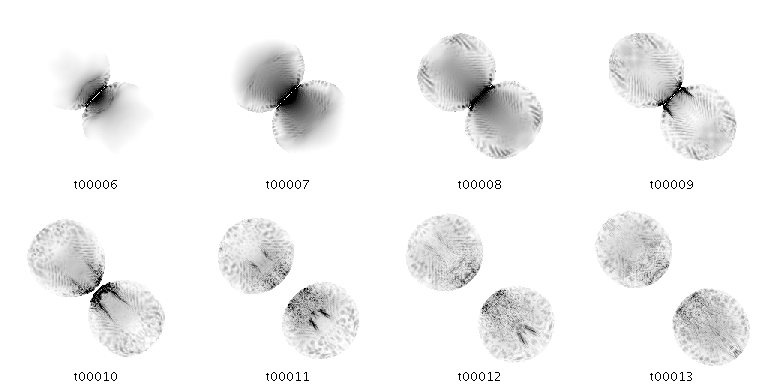
\includegraphics[scale=.60]{particle2tiff.png}
  \caption{Montage showing the averaged particle stress for two cylindrical disks colliding.}
  \label{fig:p2tiff}
\end{figure}


%__________________________________
\section{On the fly analysis} 
On the fly analysis is used to determine the minimum and maximum of specified variables while the simulation is running.  Parameters are included in the input file to specify at what frequency the data is analyzed and which variables to look at. A new directory will be made in the uda directory for each level (e.g. L-0). Within the new directory the max and min of each variable for the specified material is determined as a function of time at the given sampling frequency. 

\begin{center}
\begin{tabular}{| l | c | p{7cm} |}
\hline
  \multicolumn{3}{|c|}{\textbf{Dynamic Output Intervals Input Parameters}} \\
\hline
\hline
  \textbf{Tag} & \textbf{Type} & \textbf{Description}\\
\hline
  $<$samplingFrequency$>$ & double & Sampling frequency in times per simulated second\\
\hline
  $<$timeStart$>$ & double & Simulation time when sampling begins (sec)\\
\hline
  $<$timeEnd$>$ & double & Simulation time when sampling ends (sec)\\
\hline
  $<$Variables$>$ & String & Variables to be analyzed including a specification for which material\\
\hline
\end{tabular}
\end{center}


The input file specification is as follows:
\begin{lstlisting}
<DataAnalysis>
  <Module name = "minMax">
    <samplingFrequency> 1e8 </samplingFrequency>
    <timeStart> 0 </timeStart>
    <timeEnd> 1000 </timeEnd>
    <Variables>
      <analyze label="press_CC" matl="0"/>
      <analyze label="vel_CC" matl="1"/>
      <analyze label="rho_CC" matl="0"/>
    </Variables>
  </Module>
</DataAnalysis>
\end{lstlisting}


%\section{compare_uda}

%__________________________________
%\section{plotting tools}
% - plotStats\\
% - plotRegridder \\
% - plotCPU_usage \\
% - plotComponents

%__________________________________
%FIXME
%\subsection{Code}
%-explain the basic directory structure of src
%\begin{lstlisting}
%|-- CCA
%|-- Components
%|   |-- Angio
%|   |-- Arches
%|   |-- DataArchiver
%|   |-- Examples
%|   |-- ICE
%|   |-- LoadBalancers
%|   |-- MPM
%|   |-- MPMArches
%|   |-- MPMICE
%|   |-- Models
%|   |-- OnTheFlyAnalysis
%|   |-- Parent
%|   |-- PatchCombiner
%|   |-- ProblemSpecification
%|   |-- Regridder
%|   |-- Schedulers
%|   |-- SimulationController
%|   |-- Solvers
%|   |-- SpatialOps
%|   `-- SwitchingCriteria
%|-- Ports
%|-- Core
%|-- R_Tester
%|-- StandAlone
%|-- Teem
%|-- VisIt
%|-- build_scripts
%|-- include
%|-- orderAccuracy
%|-- scripts
%|-- tau
%|-- testprograms
%`-- tools
%\end{lstlisting}
